\documentclass[a4paper,12pt]{article} \usepackage{graphicx}
\usepackage{epstopdf} %\usepackage{gensymb} \usepackage{longtable}
\usepackage{graphicx}
%% Definitioner för LIPS-dokument

\usepackage[english,swedish]{babel}
\usepackage[utf8]{inputenc}
\usepackage[T1]{fontenc}
\usepackage{times}
\usepackage{ifthen}

\usepackage[margin=25mm]{geometry}

\usepackage{fancyhdr}
\pagestyle{fancy}
\lhead{}
\chead{\textbf{\LIPSprojekttitel}}
\rhead{\textbf{\textsl{LiTH}}\\\textbf{\LIPSdatum}}
\lfoot{\textbf{\LIPSkursnamn}\\\textbf{\LIPSdokumentansvarig}}
\cfoot{\textbf{\LIPSprojektgrupp}\\\textbf{\LIPSgruppepost}}
\rfoot{\textbf{\textsc{Lip}s}\\\textbf{Sida~\thepage}}

\setlength{\parindent}{0pt}
\setlength{\parskip}{1ex plus 0.5ex minus 0.2ex}


\newcommand{\twodigit}[1]{\ifthenelse{#1<10}{0}{}{#1}}
\newcommand{\dagensdatum}{\number\year-\twodigit{\number\month}-\twodigit{\number\day}}

%% ------------------------------------------
% NYBILD
% Skapar centrerad bild med caption
%   
% #1: Filens url relativt '/bilder/'
% #2:  Caption
% #3: Label
% #4: Skalning
%% ------------------------------------------
\newcommand{\nyBild}[4] 
{\begin{figure}[H]
  \centering
 \includegraphics[angle=0,scale=#4]{bilder/#1}
  \caption{#2}
  \label{fig:#3}
\end{figure}}



%%  Redefinitions of commands containing @
\makeatletter
\makeatother

\newcommand{\LIPStitelsida}{%
{\ }\vspace{45mm}
\begin{center}
  \textbf{\Huge \LIPSdokumenttyp}
\end{center}
\begin{center}
  {\Large Editor: \LIPSredaktor}
\end{center}
\begin{center}
  {\Large \textbf{Version \LIPSversion}}
\end{center}
\vfill
\begin{center}
  {\large Status}\\[1.5ex]
  \begin{tabular}{|*{3}{p{40mm}|}}
    \hline
    Reviewed & \LIPSgranskare & \LIPSgranskatdatum \\
    \hline
    Approved & \LIPSgodkannare & \LIPSgodkantdatum \\
    \hline
  \end{tabular}
\end{center}
\newpage
}


\newenvironment{LIPSprojektidentitet}{%
{\ }\vspace{45mm}
\begin{center}
  {\Large PROJECT IDENTITY}\\[0.5ex]
  {\small
  \LIPSartaltermin, \LIPSprojektgrupp\\
  Linköpings Tekniska Högskola, ISY
  }
\end{center}
\begin{center}
  {\small Group member}\\
%  \begin{tabular}{|p{30mm}|p{40mm}|p{35mm}|p{45mm}|}
  \begin{tabular}{|l|p{45mm}|p{25mm}|l|}
    \hline
    \textbf{Name} & \textbf{Responsibility} & \textbf{Phone} & \textbf{E-mail} \\
    \hline
}%
{%
    \hline
  \end{tabular}
\end{center}
\begin{center}
  {\small
    %\textbf{E-postlista för hela gruppen}: \LIPSgruppepost\\
    %\textbf{Hemsida}: \LIPSgrupphemsida\\[1ex]
    \textbf{Customer}: \LIPSkund\\
    \textbf{Customer Contact}: \LIPSkundkontakt\\
    \textbf{Course Leader}: \LIPSkursansvarig\\
    \textbf{Tutor}: \LIPShandledare\\
  }
\end{center}
\newpage
}
\newcommand{\LIPSgruppmedlem}[4]{\hline {#1} & {#2} & {#3} & {#4} \\}



\newenvironment{LIPSdokumenthistorik}{%
\begin{center}
  Document history\\[1ex]
  \begin{small}
    \begin{tabular}{|l|l|p{60mm}|l|l|}
      \hline
      \textbf{Version} & \textbf{Date} & \textbf{Changes} & \textbf{Edited by} & \textbf{Reviewed} \\
      }%
    {%
      \hline
    \end{tabular}
  \end{small}
\end{center}
}
\newcommand{\LIPSversionsinfo}[5]{\hline {#1} & {#2} & {#3} & {#4} & {#5} \\}

\newcounter{LIPSkravnummer}
\newcounter{LIPSunderkravnummer}[LIPSkravnummer]

\newenvironment{LIPSkravlista}{%
  \begin{tabular}{|p{25mm}|p{25mm}|p{85mm}|p{5mm}|}
    }%
  {%
    \hline
  \end{tabular}
}

\newenvironment{LIPSleveranslista}{%
  \begin{tabular}{|p{25mm}|p{20mm}|p{65mm}|p{25mm}|p{5mm}|}
    }%
  {%
    \hline
  \end{tabular}
}


\newcommand{\LIPSkrav}[3]
{\hline
\stepcounter{LIPSkravnummer}\textbf{Krav nr \arabic{LIPSkravnummer}} &
\textbf{{#1}} & 
{#2} & 
\textbf{{#3}} 
\\}

\newcommand{\LIPSleverans}[4]
{\hline
        \textbf{{#1}} & 
        {#2} & 
        {#3} & 
        \textbf {{#4}} 
\\}

\newcommand{\LIPSunderkrav}[3]{\hline\stepcounter{LIPSunderkravnummer}\textbf{Requirement nr \arabic{LIPSkravnummer}\Alph{LIPSunderkravnummer}} & \textbf{{#1}} & {#2} & \textbf{{#3}} \\}





%%% Local Variables: 
%%% mode: latex
%%% TeX-master: "kravspec_mall"
%%% End: 


\newcommand{\degree}{\ensuremath{^\circ}}
\newcommand{\LIPSartaltermin}{2013/VT}
\newcommand{\LIPSkursnamn}{TSEK06}
\newcommand{\LIPSprojekttitel}{DLL Based Frequency Multiplier}

\newcommand{\LIPSprojektgrupp}{Group 7}

\newcommand{\LIPSgruppepost}{}
\newcommand{\LIPSgrupphemsida}{} 
\newcommand{\LIPSdokumentansvarig}{Gustav Svensk}

\newcommand{\LIPSkund}{ISY, Linköpings universitet, 581\,83 Linköping}

\newcommand{\LIPSkundkontakt}{Amin Ojani}
\newcommand{\LIPSkursansvarig}{Atila Alvandpour}
\newcommand{\LIPShandledare}{Amin Ojani}



\newcommand{\LIPSdokumenttyp}{High Level Simulation} 
\newcommand{\LIPSredaktor}{Nora Björklund} 
\newcommand{\LIPSversion}{0.1} 
\newcommand{\LIPSdatum}{\dagensdatum}

\newcommand{\LIPSgranskare}{} 
\newcommand{\LIPSgranskatdatum}{}
\newcommand{\LIPSgodkannare}{} 
\newcommand{\LIPSgodkantdatum}{}

\begin{document}
\LIPStitelsida

%% Argument till \LIPSgruppmedlem: namn, roll i gruppen, telefonnummer, epost
\selectlanguage{swedish}
\begin{LIPSprojektidentitet}
 
\LIPSgruppmedlem{Nora Björklund}{Project leader}{076 7756
789}{norbj648@student.liu.se}
\LIPSgruppmedlem{\LIPSdokumentansvarig}{Documentation}{073
6208776}{grulfen3@gmail.com} 
\LIPSgruppmedlem{Christopher Hallberg}{}{0739845945}{chrha007@student.liu.se} 
\LIPSgruppmedlem{Gustaf Bengtz}{}{07073607307}{gbengtz@gmail.com} 
\LIPSgruppmedlem{Johan Berneland}{}{0704988329}{johbe915@student.liu.se}
\end{LIPSprojektidentitet}


\selectlanguage{english}

\tableofcontents{} 
\newpage %% Argument till \LIPSversionsinfo: versionsnummer, datum, Ändringar,
         %  utfört av,granskat av
\addcontentsline{toc}{section}{Document history} \begin{LIPSdokumenthistorik} 
\LIPSversionsinfo{0.1}{}{First draft.}{}{}\end{LIPSdokumenthistorik} 
\newpage


\section{Overview}
An overview of the system can be seen in \ref{fig:system}.
\begin{figure}[h]
        \centering
        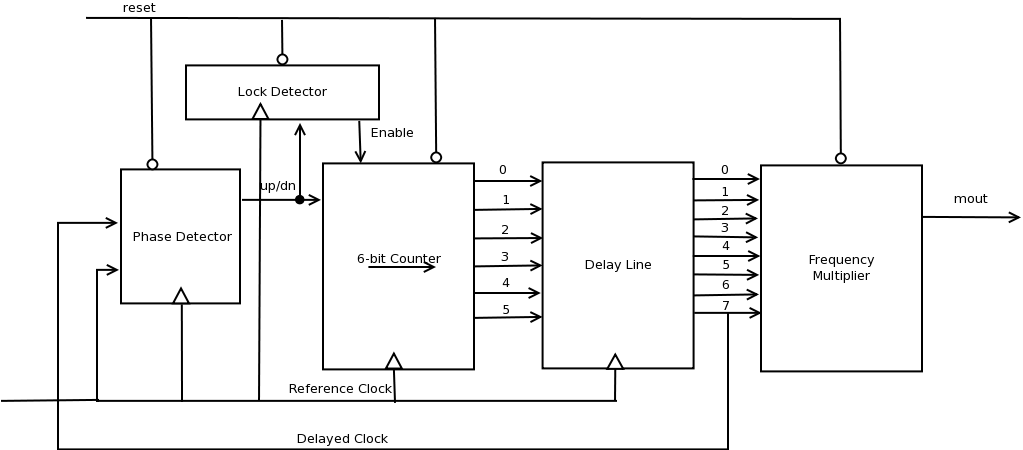
\includegraphics[width=150mm]{../Bilder/hll_system.png}
        \caption{Overview of the system}
        \label{fig:system}
\end{figure}
\section{Block Level and Description}
In the subsections below the blocks presented above will be described in detail.

\subsection{Phase Detector}
The phase detector (PD) has a very simple design. It is a DFF with the
reference clock as update signal and the delayed clock signal coming
out from the delay cells as input signal. If the delayed clock rises before
the reference clock does, the output will be set to a logic high resulting it to 
be more delayed since it rose too early. If the delayed clock has not yet risen 
when the reference clock rises the output will be set to a logic zero, causing 
it to be less delayed. The clocks are checked when the transient voltage (i.e 50\% 
of rise-time/fall-time) is exceeded.
 
\subsection{Counter}
The counter takes an input from the PD and either increments
the internal value, or decrements it. If the input from the PD is one the
counter is incremented, and decresed if the input is zero. The counter also has
an enable signal coming from the lock-detector. If the enable is high the counter
is active, and it is inactive when the enable is low. This is implemented to 
save power, and avoid the toggle state that the counter is bound to end up in when
the phases between the reference clock and the delayed clock match.


\subsection{Delay Line}
The delay block will in the finished design consist of eight inverter cells,
each delaying the signal 45\degree giving a total delay of 360\degree. In turn
each inverter cell might consist of an odd number of smaller inverters to buffer
the signal in order to obtain better rise and fall times.

However, in the high level implementation the delay cells are modeled
as a single block consisting of Verilog A code. To model the inverter
cells the input clock signal is inverted eight times and the intermediate
signals are put on the output. Each of the inverters have a rise and a
fall time of 100ps to simulate physical properties. They also have an
inherent delay of 400ps. For now these numbers are just parameters set
in the Verilog A code but will later on in the project be determined
by sizing of transistors, capacitance among other things.

To be able to tune the delay for a given input signal an extra
variable delay is needed for each inverter. On transistor level this
will be done by switching on and off binary weighted capacitive loads,
but in the high level design these are just delays set explicit as time
values. How many of these binary weighted delays should be active at a
given time is controlled by the input to the delay line from the 6-bit
counter, as can be seen in \ref{fig:system}. 


\subsection{Lock-detector}
The lock-detector takes the output signal from the Phase Detector and uses
it to check if the Phase Detector has reached the toggle state or not. If the Phase
Detector send an alternation of increment and decrement instructions to the counter
seven times the Phase Detection is considered to be done and the enable 
signal sent to the counter is put to low. This forces the counter to lock its 
current value which locks the delay.


\subsection{Frequency Multiplier}
The frequency multiplier contains 3 blocks, one 8-input multiplexer, one 3-bit
counter and one 3-input multiplexer, the blocks and connections can be seen in 
figure \ref{fig:freq_mult}.
\begin{figure}[h!b]
        \centering
        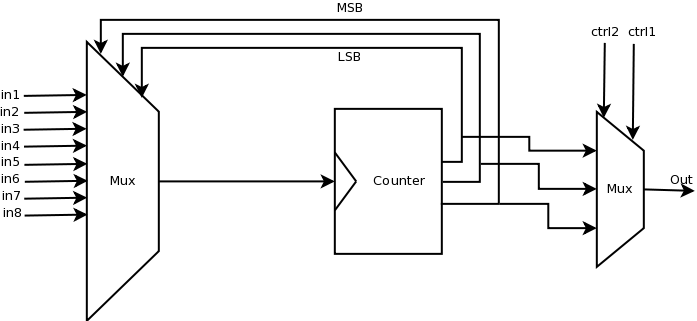
\includegraphics[width=0.6\textwidth]{../Bilder/freq_mult_high.png}
        \caption{Frequency Multiplier}
        \label{fig:freq_mult}
\end{figure}
The eight delayed versions of the input signal from the delay cells
are the inputs to the 8-input multiplexer, each signal delayed 45\degree 
compared to the previous one. The output of the 8-input multiplexer is 
connected to the clock of the counter and the output of the counter is 
controlling the 8-input multiplexer. So when a rising edge on the clock
makes the counter tick once, the new clock signal is a 45\degree shifted
version of the previous one, making the counter tick 4 times faster than
if the input signal was used as clock. The 3-input multiplexer chooses which 
signal it to be used as output, bit one, two or three of the counter output. 
In table \ref{tab:mult_fact} the different control signals to choose 
multiplication factor can be seen.
\begin{table}[h!]
        \centering
        \begin{tabular}{|c|c|}
                \hline
                \textbf{Control signals} & \textbf{Multiplication factor} \\
                \hline
                00 & 1 \\
                01 & 2 \\
                10 & 2 \\
                11 & 4 \\
                \hline
        \end{tabular}
        \caption{Multiplication Factors}
        \label{tab:mult_fact}
\end{table}

\section{Simulation Result}
The simulation result of the whole system and the individual Blocks is
presented below.
\subsection{Whole System Simulation}
Simulation of the whole system with a 250 MHz input signal successfully
generates an output of 1 GHz, this can be seen in figure \ref{fig:high_sim}.
It can be noted that it takes a while for the system to produce a good output
with around 50\% duty cycle, this is because it takes some time for the DLL
to lock.
\begin{figure}[hb]
        \centering
        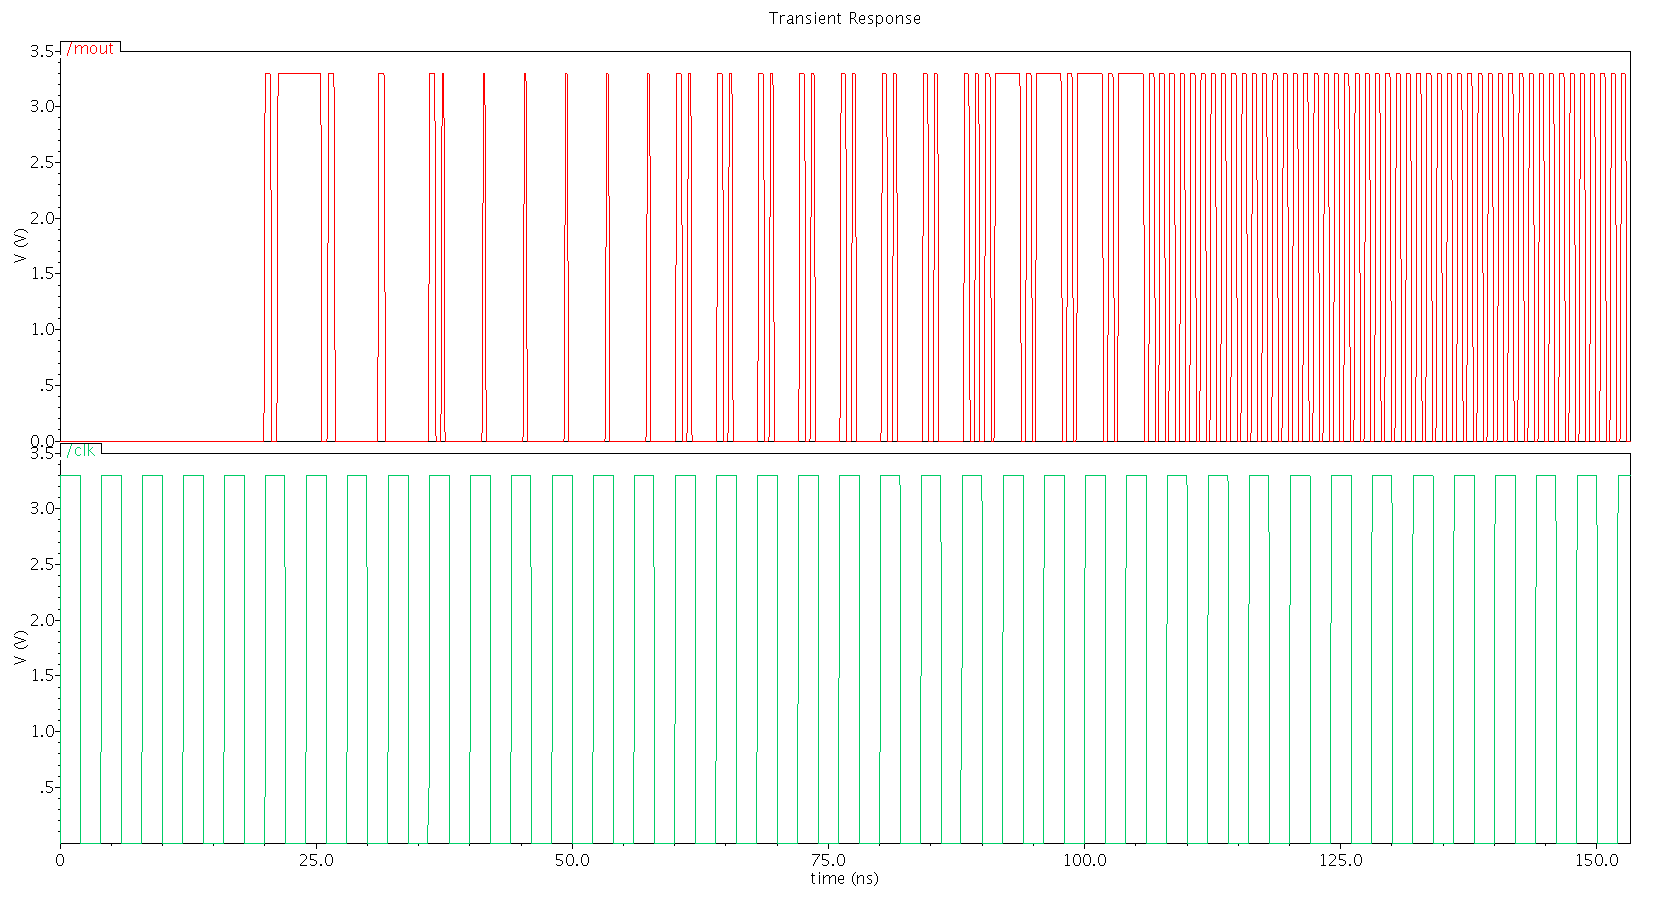
\includegraphics[width=\textwidth]{../Bilder/high_level_sim.png}
        \caption{Simulation of the whole system}
        \label{fig:high_sim}
\end{figure}

%% Insert each blocks's simulation result here
\subsection{Phase Detector}
\subsection{Counter}
\subsection{Delay Line}
Simulating the delay line in high level is mostly just a matter of
seeing if the Verilog A code is correct. Since there are no physical
considerations to take into account at this stage thorough simulations
on the delay line alone are of little interest. It is, however, useful
to get a visualization of the delayed signals and the tuning of this
delay. When deciding on the resolution of the variable delay
controlled by the 6-bit counter some consideration needs to be taken. 
There is a trade-off between resolution and the
range of possible input frequencies. Simulations showed this very
clearly. 

Simulation was performed with different values on the variable
delay. The target input frequency is 250MHz so focus is placed to make
the delay line work well near this value. Finally the inherent fixed
delay of the inverters was set to 400ps, as mentioned in the
description of the delay block, and the
LSB of the variable delay was set to 5ps. This gives a resolution of
40ps on the whole delay line. The range of possible input frequency
will with this resolution be approximately 166-278MHz. This was
verified by the simulation results.
\subsection{Frequency Multiplier}

\section{Risks and Delays}
%% nämn övergripande process variations. typ vad det är för ngt
%%ska detta vara här? är det denna typen av ``risks and delays'' som
%%efterfrågas? om ni vill kan ni slå ihop min subsection under section.
\subsection{Delay Line}
A problem with process variation for the delay line is that the delay
needs to be very exact in order for the whole thing to work. If the
fixed delay of each inverter cell is off-set when the chip is
delivered the variable delay needs to be able to handle this. Also,
if by chance the target input frequency needs to be lowered the delay
needs to be long enough to handle this. If focus is on only making it
perform well at 250MHz it might not work with a lower frequency. 

Also, in the high level design the delay is explicitly determined by
the time values set in the Verilog A file. Later on the delay needs to
be set by transistor sizing and the capacitance. Things like
non-linearities needs to be considered.
\end{document} 

%%% Local Variables: %%% mode: latex %%% TeX-master: t %%% End:
